\documentclass{amsart}

\usepackage[utf8]{inputenc}
\usepackage[T2A]{fontenc}
\usepackage[english,russian]{babel}
\usepackage{amsthm,amsmath,amsfonts,amssymb}
\usepackage{fullpage}
\usepackage{eufrak}

%%% Дополнительная работа с математикой
\usepackage{amsfonts,amssymb,amsthm,mathtools} % AMS
\usepackage{amsmath}
\usepackage{icomma}

%% Шрифты
\usepackage{euscript}	 % Шрифт Евклид
\usepackage{mathrsfs} % Красивый матшрифт

%% Свои команды
\DeclareMathOperator{\sgn}{\mathop{sgn}}	% сигнум
\DeclareMathOperator{\cov}{\mathop{cov}}	% ковариация
\DeclareMathOperator{\lb}{\mathop{lb}}	% бинарный логарифм (логарифм по основанию 2)
\DeclareMathOperator{\supp}{\mathop{supp}}	% носитель

\renewcommand{\Im}{\mathop{\mathrm{Im}}\nolimits}	% мнимая часть
\renewcommand{\Re}{\mathop{\mathrm{Re}}\nolimits}	% вещественная часть

\renewcommand{\Prob}{\mathbb P}	% вероятность
\newcommand{\Expect}{\mathbb E}	% математическое ожидание
\renewcommand{\Variance}{\mathbb D}	% дисперсия
\newcommand{\Entropy}{\mathbb H}	% энтропия

%% Перенос знаков в формулах (по Львовскому)
\newcommand*{\hm}[1]{#1\nobreak\discretionary{}
	{\hbox{$\mathsurround=0pt #1$}}{}}

%%% Работа с картинками
\usepackage{graphicx}  % Для вставки рисунков
\graphicspath{{images/}{images2/}}  % папки с картинками
\setlength\fboxsep{3pt} % Отступ рамки \fbox{} от рисунка
\setlength\fboxrule{1pt} % Толщина линий рамки \fbox{}
\usepackage{wrapfig} % Обтекание рисунков и таблиц текстом
\RequirePackage{caption}
\DeclareCaptionLabelSeparator{defffis}{ -- }
\captionsetup{justification=centering,labelsep=defffis}

\renewcommand{\qedsymbol}{}

%%% Работа с таблицами
\usepackage{array,tabularx,tabulary,booktabs} % Дополнительная работа с таблицами
\usepackage{longtable}  % Длинные таблицы
\usepackage{multirow} % Слияние строк в таблице

\newtheorem*{problem}{Задание}

\begin{document}
	
	\newcommand{\problemset}[1]{
		\begin{center}
			\Large #1
		\end{center}
	}
	
	\begin{tabbing}
	\hspace{11cm} \= Студент: \= Ибрагимов Эдгар \\ % не забудьте исправить, студент Вы или студентка :) % (а то некоторые забывают)
	\> Группа: \> 2303 \\  % Здесь меняете № группы
	\> Вариант: \> 6 \\    % А здесь меняете № варианта
	\> Дата: \> \today     % А вот здесь ничего не меняем!!!
\end{tabbing}
\hrule
\vspace{1cm}  % в данном файле меняем только Пол, Фамилию Имя, № группы и № варианта
	\problemset{Комбинаторика и теория графов}
\problemset{Индивидуальное домашнее задание №1}	% поменяйте номер ИДЗ

\renewcommand*{\proofname}{Решение}

%%%%%%%%%%%%%% ЗАДАНИЕ №2 %%%%%%%%%%%%%%
%% Условие задания №2
\begin{problem}[2]
	Найдите а) наименьшее; б) наибольшее возможное количество компонент связности в графе с 15 вершинами и 16 рёбрами.
\end{problem}

%% Решение задания №2
\begin{proof}
    а) Рассмотрим простую цепь из 15 вершин, для построения которой нам нужно 14 рёбер. Полный же граф \(K_{15}\) требует \(\frac{n(n - 1)}{2} = \frac{15\cdot{14}}{2} = 105\) вершин. Значит может существовать связный граф из 15 вершин и 16 рёбер, то есть минимальной число компонент связности равно 1.

    б) Для того чтобы определить максимально возможное число компонент связности для графа, найдем такой наименьший полный граф, что количество его рёбер не менее $16$: $\frac{n(n - 1)}{2} \geqslant 16$ $\Rightarrow$ $n = 7$. Рассмотрим $15 - 7 = 8$ компонент связностей, которые являются изолированными вершинами, а 9-я имеет 7 вершин и 16 рёбер. Действительно, число компонент связностей графа должно равняться $\upsilon - n + 1 = 15 - 7 + 1 = 9$

    Ответ: a) 1, б) 9.
\end{proof}

%%%%%%%%%%%%%% ЗАДАНИЕ №3 %%%%%%%%%%%%%%
%% Условие задания №3
\begin{problem}[3]
	В задании могут быть использованы петли.
    
    а) Существует ли граф со степенями вершин 1, 4, 4, 1, 5, 6, 3? Если существует, постройте его, если нет - объясните почему.
    
    б) Существует ли граф со степенями вершин 0, 3, 3, 0, 4, 5, 2? Если существует, постройте его, если нет - объясните почему.
\end{problem}

%% Решение задания №3
\begin{proof}
    а) По лемме о рукопожатиях $E = \frac{1}{2}\sum\limits_{i=1}^{n}deg(V_{i})$ = 12 - число целое , такой конечный граф существует. Пример:

    \begin{figure}[h]
    \centering
     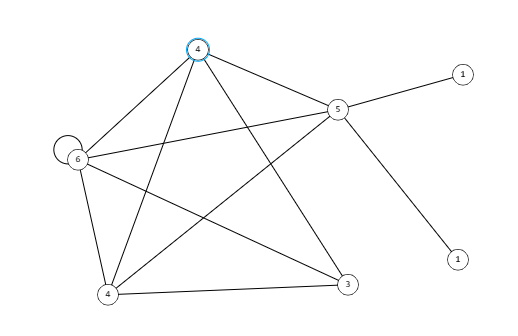
\includegraphics[width=0.6\linewidth]{pics/3_a_solution.png}
     \label{fig:dm}
    \end{figure}

    б) По лемме о рукопожатиях, для существования конечного графа число вершин с нечетной степенью должно быть четно. В рассматриваемом случае количество таких вершин 3, 3, 5 - нечётно. Следовательно такого графа не существует.
\end{proof}

%%%%%%%%%%%%%% ЗАДАНИЕ №5 %%%%%%%%%%%%%%
%% Условие задания №5
\begin{problem}[5]
	Является ли граф: 
    \begin{figure}[h]
    \centering
     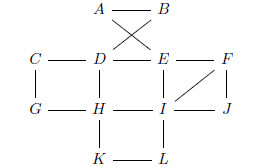
\includegraphics[width=0.4\linewidth]{pics/Graph5th.png}
     \label{fig:dm}
    \end{figure}
    
    а) эйлеровым, полуэйлеровым?
    
    в) двудольным?
\end{problem}

%% Решение задания №5
\begin{proof}
	а) Граф является полуэйлеровым, поскольку он связный и имеет ровно 2 вершины F, I с нечетной степенью.

    \begin{figure}[h]
    \centering
     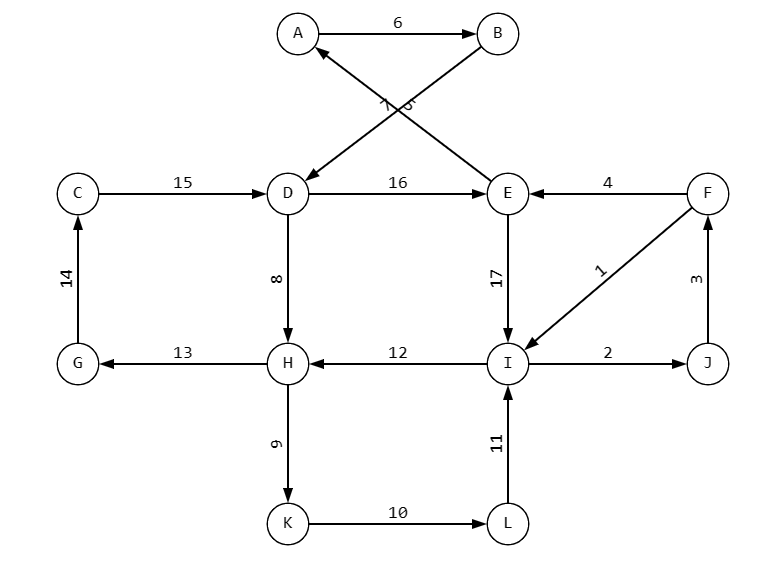
\includegraphics[width=0.45\linewidth]{pics/5th_a_solution.png}
     \label{fig:dm}
    \end{figure} 
\end{proof}
    в) Граф не является двудольным, поскольку вершины F, I, J образуют циклл нечетной длины.
    
%%%%%%%%%%%%%% ЗАДАНИЕ №8 %%%%%%%%%%%%%%
%% Условие задания №8
\begin{problem}[8]
	При помощи алгоритма Kosaraju найдите компоненты сильной связности данного графа:
 
    \begin{figure}[h]
    \centering
     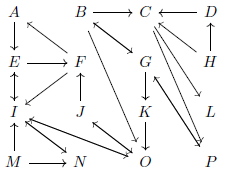
\includegraphics[width=0.3\linewidth]{pics/Graph8th.png}
     \label{fig:dm}
    \end{figure}

    Постройте граф конденсации
\end{problem}

%% Решение задания №8
\begin{proof}
 Для удобства изменив представление графа - Рис. 1.
 
    \begin{figure}[h]
    \centering
     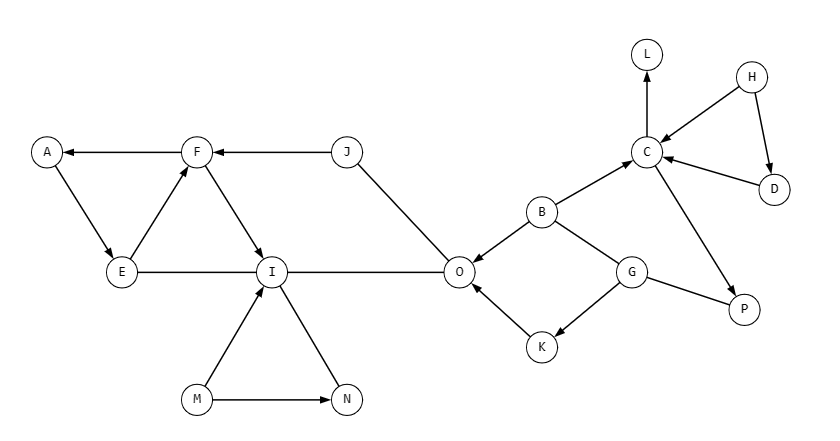
\includegraphics[width=0.7\linewidth]{pics/8thGraphSol.png}
     \label{fig:dm}
     \caption{Изменённый граф}
    \end{figure}
 
 Проходимся по графу с помощью алгоритма DFS:
 
 Очередь: HCLPGBOJFAEINKDM\\

 Инвертируем направление рёбер - Рис. 2.

 \begin{figure}[h]
    \centering
     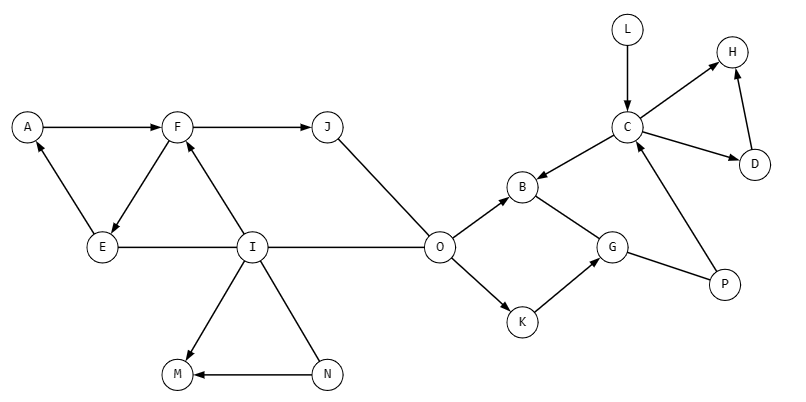
\includegraphics[width=0.7\linewidth]{pics/8thInverGraph.png}
     \label{fig:dm}
     \caption{Граф с инвертированными направлениями дуг}
    \end{figure}
 
 Применяем алгоритм DFS ещё раз соблюдая предыдущую очередь выбора вершин:\\
 
 Очередь: MDHKCBPCNIEAFJOL

 Получаем лес: M, DH, KGBPC, NIEAFJO, L - искомые компоненты сильной связности.
 
 В результате строим по ним граф конденсации - Рис. 3.

 \begin{figure}[h]
    \centering
     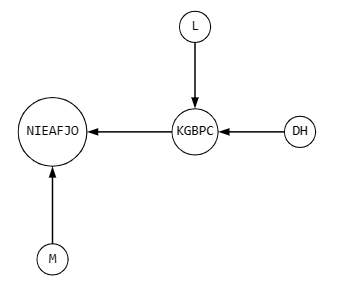
\includegraphics[width=0.3\linewidth]{pics/8thCondensGraph.png}
     \label{fig:dm}
     \caption{Граф конденсации}
    \end{figure}
\end{proof}

%%%%%%%%%%%%%% ЗАДАНИЕ №16 %%%%%%%%%%%%%%
%% Условие задания №16
\begin{problem}[16]
	а)При помощи алгоритма Прима или Краскала найдите минимальное остовное дерево данного графа:\\
    \begin{figure}[h]
    \centering
     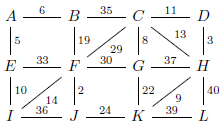
\includegraphics[width=0.35\linewidth]{pics/Graph16th.png}
     \label{fig:dm}
    \end{figure}
    
\end{problem}

%% Решение задания №16
\begin{proof}
    Выпишем все рёбра графа в отсортированном порядке:

    F <--> J : w = 2

    D <--> H : w = 3 

    A <--> E : w = 5 

    A <--> B : w = 6 

    C <--> G : w = 8

    H <--> K : w = 9

    E <--> I : w = 10

    C <--> D : w = 11

    C <--> H : w = 13

    F <--> I : w = 14

    B <--> F : w = 19

    G <--> K : w = 22

    J <--> K : w = 24

    C <--> F : w = 29

    F <--> G : w = 30

    E <--> F : w = 33

    B <--> C : w = 35

    I <--> J : w = 36

    G <--> H : w = 37

    K <--> L : w = 39

    H <--> L : w = 40

    И начнем по списку добавлять эти ребра в наш остов, так чтобы при добавлении следующего не образовывались циклы. В итоге получился остов:

    \begin{figure}[h]
    \centering
     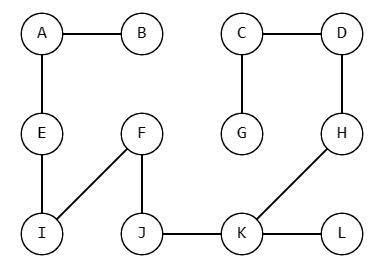
\includegraphics[width=0.35\linewidth]{pics/16th_a_solution.png}
     \label{fig:dm}
    \end{figure}
\end{proof}  % для удобства создаём по аналогии файлы ihw1.tex, ihw2.tex, etc
	                  % и просто меняем имя при компиляции
\end{document}